\chapter{Worksheet}
\section{Friis}

The reason why there is a loss through free space, is that the signal density gets lower, as it spread over a larger area, which happens when the distance, that the signal has travelled, gets longer. 

A example, is when using a isotropic antenna, the signal density is equal all the way around the antenna, forming a sphere around the antenna. As the power of the signal in total always is the same, the density of the signal power is depended on the surface of the sphere. As the signal travels longer away from the antenna, the sphere gets bigger and the surface bigger to, which means that the signal density gets lower. So the free space loss, is the factor describing the signal that is not going in the direction of the receiving antenna.


Friis transmission equation is used to calculate the power, that is received at the receiving antenna, out from the gains in the antenna, the power of the transmitted signal and the free space loss. 

\begin{equation}
P_r = P_t G_t G_r (\frac{\lambda}{4 \pi d})^2
\end{equation}
\begin{where}
\va{$P_r$}{is the received power at the receiving antenna}{W}
\va{$P_r$}{is the transmitted power at the transmitting antenna}{W}
\va{$G_t$}{is the gain in the transmitting antenna}{1}
\va{$G_r$}{is the gain in the receiving antenna}{1}
\va{$\lambda$}{is the wavelength of the transmitted signal}{m}
\va{$d$}{is the distance between the transmitting antenna and the receiving antenna}{m}
\end{where}

It is used to calculate the loss through the free space and does not take into account other waves, than the direct wave. The free space loss is equal to $(\frac{\lambda}{4 \pi d})^2$ and is multiplied by the gains in both antennas and the power transmitted, to get the received power level.

The free space loss comes from the spreading of the signal, which is compared to the spheres, which in the signal spread in, surface, which is calculated by $\frac{1}{4 \pi d^2}$. Furthermore, there also comes the loss, when the signal is received at the receiver, where the effective antenna area is equal to $\frac{\lambda^2}{4 \pi}$. These two losses give in total the free space loss. (Hans eberts pdf)


This is the simple form of friis formulae and it is only correct, if these conditions is met:
\begin{itemize}
\item $d$ is much greater than $\lambda$. If $d$ is smaller than $\lambda$, there will be gain in power through the transmission between the antennas, which is a violation of the law of conservation of energy.
\item The transmission goes through freespace, with no multipath. So no obstacle in the transmission line or around it (See worksheet about Line of sight (LOS)).
\item The antennas is aligned and have the same polarization.
\item The bandwidth is narrow enough, so that a single wavelength can be specified.
\item $P_r$ and $P_t$ is the available power at the antennas, and do not take into account the loss through the cable running from antennas. Furthermore, the power will only be fully delivered and received, if the antennas and transmission lines are conjugate matched.
\end{itemize}


When the antennas are not aligned and/or do not have the same polarization, the simple version of the equation cannot be used. Another problem, is if the impedances is mismatched, which gives a reflection at the antennas, which is another loss in the system. Also there is loss through the air, where the air absorb some of the power from the signal. With these losses, the equation is expanded to:

\begin{equation}
P_r = P_t G_t(\theta_t, \phi_t) G_r(\theta_r, \phi_r) (\frac{\lambda}{4 \pi d})^2 (1 - \mid \Gamma_t \mid^2) (1 - \mid \Gamma_r \mid^2) \mid a_t \cdot a_r^* \mid^2 e^{- \alpha d}
\end{equation}
\begin{where}
\va{$P_r$}{is the received power at the receiving antenna}{W}
\va{$P_r$}{is the transmitted power at the transmitting antenna}{W}
\va{$G_t(\theta_t, \phi_t)$}{is the gain in the transmitting antenna}{1}
\va{$G_r(\theta_t, \phi_t)$}{is the gain in the receiving antenna}{1}
\va{$\lambda$}{is the wavelength of the transmitted signal}{m}
\va{$d$}{is the distance between the transmitting antenna and the receiving antenna}{m}
\va{$\Gamma_t$}{is the reflection constant a the transmitting antenna}{1}
\va{$\Gamma_r$}{is the reflection constant a the receiving antenna}{1}
\va{$a_t$}{is the polarization vector of the transmitting antenna}{1}
\va{$a_r$}{is the polarization vector of the receiving antenna}{1}
\va{$\alpha$}{is the medium of transportations absorption coefficient}{1}
\end{where}

The new terms comes from different losses in the system, when the system is not ideal.


%\begin{figure}[H]
%\centering
%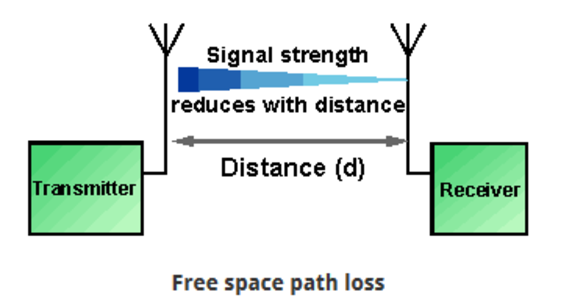
\includegraphics[width=0.6\textwidth]{freespace_fig.pdf}
%\caption{Illustration of Near field and Far field \citep{farnear_field}}
%\label{para_wave}
%\end{figure}

